\documentclass{beamer}

\usepackage{comment}
\usepackage{color}
\usepackage{listings}
\usepackage{verbatim}
\usepackage{multicol}
\usepackage{booktabs}
\definecolor{green}{RGB}{0,128,0}

\def\EQ#1\EN{\begin{equation*}#1\end{equation*}}
\def\BA#1\EA{\begin{align*}#1\end{align*}}
\def\BS#1\ES{\begin{split*}#1\end{split*}}
\newcommand{\bc}{\begin{center}}
\newcommand{\ec}{\end{center}}
\newcommand{\eq}{\ =\ }
\newcommand{\degc}{$^\circ$C}

\def\p{\partial}
\def\qbs{\boldsymbol{q}}
\def\Dbs{\boldsymbol{D}}
\def\A{\mathcal A}
\def\gC{\mathcal C}
\def\gD{\mathcal D}
\def\gL{\mathcal L}
\def\M{\mathcal M}
\def\P{\mathcal P}
\def\Q{\mathcal Q}
\def\gR{\mathcal R}
\def\gS{\mathcal S}
\def\X{\mathcal X}
\def\bnabla{\boldsymbol{\nabla}}
\def\bnu{\boldsymbol{\nu}}
\renewcommand{\a}{{\alpha}}
%\renewcommand{\a}{{}}
\newcommand{\s}{{\sigma}}
\newcommand{\bq}{\boldsymbol{q}}
\newcommand{\bz}{\boldsymbol{z}}
\def\bPsi{\boldsymbol{\Psi}}

\def\Li{\textit{L}}
\def\Fb{\textbf{f}}
\def\Jb{\textbf{J}}
\def\cb{\textbf{c}}

\def\Dt{\Delta t}
\def\tpdt{{t + \Delta t}}
\def\bpsi{\boldsymbol{\psi}}
\def\dbpsi{\delta \boldsymbol{\psi}}
\def\bc{\textbf{c}}
\def\dbc{\delta \textbf{c}}
\def\arrows{\rightleftharpoons}

\newcommand{\bGamma}{\boldsymbol{\Gamma}}
\newcommand{\bOmega}{\boldsymbol{\Omega}}
%\newcommand{\bPsi}{\boldsymbol{\Psi}}
%\newcommand{\bpsi}{\boldsymbol{\psi}}
\newcommand{\bO}{\boldsymbol{O}}
%\newcommand{\bnu}{\boldsymbol{\nu}}
\newcommand{\bdS}{\boldsymbol{dS}}
\newcommand{\bF}{\boldsymbol{F}}
\newcommand{\bg}{\boldsymbol{g}}
\newcommand{\bJ}{\boldsymbol{J}}
\newcommand{\bk}{\boldsymbol{k}}
%\newcommand{\bq}{\boldsymbol{q}}
\newcommand{\br}{\boldsymbol{r}}
\newcommand{\bR}{\boldsymbol{R}}
\newcommand{\bS}{\boldsymbol{S}}
\newcommand{\bu}{\boldsymbol{u}}
\newcommand{\bv}{\boldsymbol{v}}
%\newcommand{\bz}{\boldsymbol{z}}
\newcommand{\pressure}{P}

\def\water{H$_2$O}
\def\calcium{Ca$^{2+}$}
\def\copper{Cu$^{2+}$}
\def\magnesium{Mg$^{2+}$}
\def\sodium{Na$^+$}
\def\potassium{K$^+$}
\def\uranium{UO$_2^{2+}$}
\def\hion{H$^+$}
\def\hydroxide{0H$^-$}
\def\bicarbonate{HCO$_3^-$}
\def\carbonate{CO$_3^{2-}$}
\def\cotwo{CO$_2$(aq)}
\def\chloride{Cl$^-$}
\def\fluoride{F$^-$}
\def\phosphoricacid{HPO$_4^{2-}$}
\def\nitrate{NO$_3^-$}
\def\sulfate{SO$_4^{2-}$}
\def\souotwooh{$>$SOUO$_2$OH}
\def\sohuotwocothree{$>$SOHUO$_2$CO$_3$}
\def\soh{$>$SOH}
\def\co2{CO$_2$}

\newcommand\gehcomment[1]{{{\color{orange} #1}}}
\newcommand\add[1]{{{\color{blue} #1}}}
\newcommand\remove[1]{\sout{{\color{red} #1}}}
\newcommand\codecomment[1]{{{\color{green} #1}}}
\newcommand\redcomment[1]{{{\color{red} #1}}}
\newcommand\bluecomment[1]{{{\color{blue} #1}}}
\newcommand\greencomment[1]{{{\color{green} #1}}}
\newcommand\magentacomment[1]{{{\color{magenta} #1}}}

\begin{comment}
\tiny
\scriptsize
\footnotesize
\small
\normalsize
\large
\Large
\LARGE
\huge
\Huge
\end{comment}

\begin{document}
\title{Supercritical \co2 Injection Scenario\ldots in a Nutshell}
\author{Satish Karra}
\date{\today}

%\frame{\titlepage}

%-----------------------------------------------------------------------------
\section{Description of Supercritical \co2 Injection}

\subsection{Supercritical \co2-water Multiphase Flow Scenario}

\frame{\frametitle{Description of \co2 Injection Flow Scenario}
The ``\co2 Injection Flow Scenario'' simulates multiphase supercritical \co2-water flow. Water is in the system initially and supercritical \co2 is injected in the center of the domain.  Assumptions include:
\begin{itemize}
  \small
  \item Problem domain: $2500 \times 2500 \times 1000$ m (x $\times$ y $\times$ z)
  \item Grid resolution $21 \times 21 \times 20$ grid cells
  \item Datum at z = 1000
  \item Hydrostatic initial and boundary conditions at 20 MPa
  \item Injection time: 20 y
  \item Supercritical \co2 injection rate: 10 kg/s
  \item Total simulation time: 100 y
\end{itemize}
}


\frame{\frametitle{Description of \co2 Injection Flow Scenario}
\begin{center}
 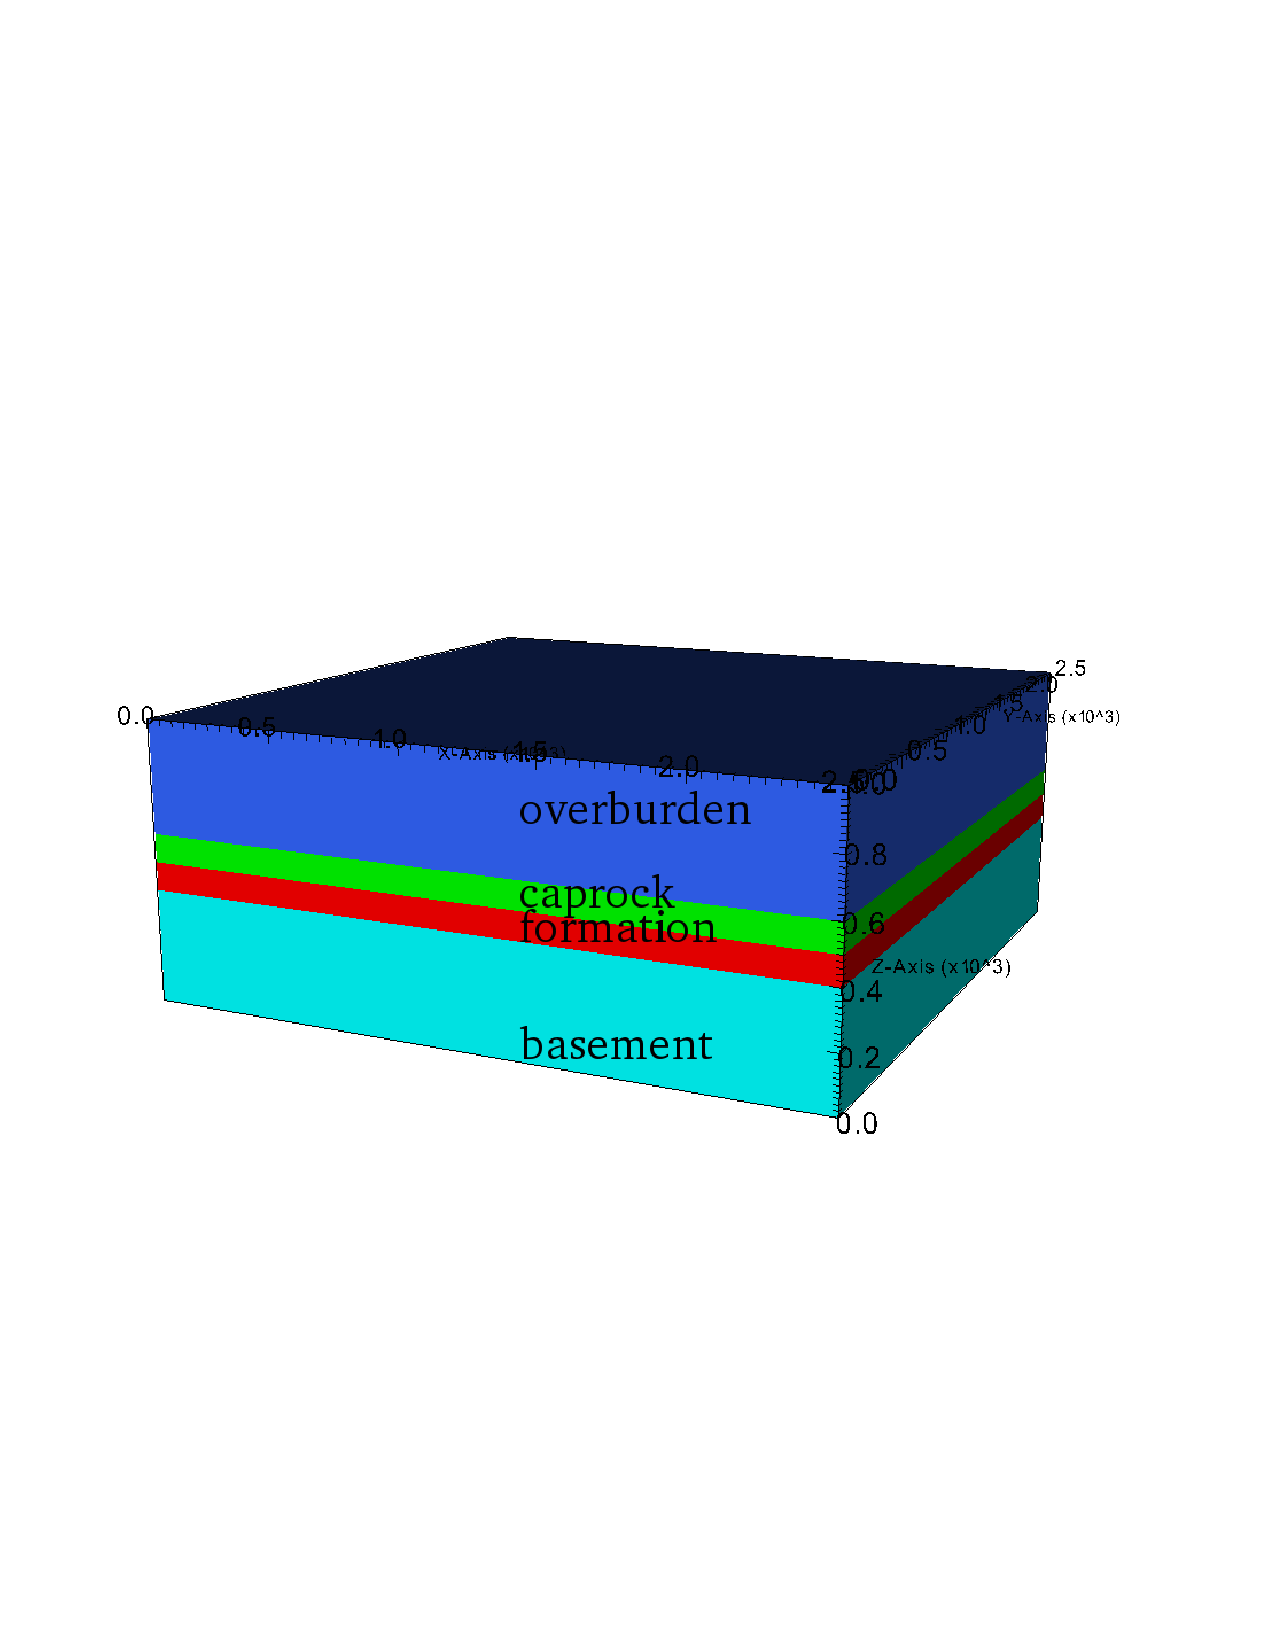
\includegraphics[width=0.85\textwidth]{./co2-schematic.pdf}
\end{center}
}

%%%%%%%%%%%%%%%%%%%%%%%%%%%%%%%%%%%%%%%%%%%%%%%%%%%%%%%%%%%%%%%%%%%%%%%%

\begin{frame}
\frametitle{\bf Governing Equations}

\begin{tabular}{lll}
{\bf Phases:} &H$_2$O ($l$); &supercritical CO$_2$ ($g$)\\
{\bf Components:} &H$_2$O ($w$); &CO$_2$ ($c$)
\end{tabular}

\medskip

\[
\begin{array}{lr}
\text{{\bf H$_2$O:}} & \dfrac{\p}{\p t} \varphi \big( s_l \rho_l X_w^l + s_g \rho_g X_w^g\big) + \bnabla\cdot \bF_w \eq Q_w,\\
~\\
\text{{\bf CO$_2$:}} & \dfrac{\p}{\p t} \varphi \big( s_l \rho_l X_c^l + s_g \rho_g X_c^g\big) + \bnabla\cdot \bF_c \eq Q_c,
\end{array}
\]

{\bf Flux:}
\vspace{-5mm}
\[
{\bF}_w \eq \bq_l \rho_l X_w^l+ \bq_g \rho_g X_w^g -\varphi s_l \rho_l D_l \bnabla X_w^l-\varphi s_g \rho_g D_g \bnabla X_w^g,
\]
\[
{\bF}_c \eq \bq_l \rho_l X_c^l+ \bq_g \rho_g X_c^g -\varphi s_l \rho_l D_l \bnabla X_c^l-\varphi s_g \rho_g D_g \bnabla X_c^g,
\]
\begin{align*}
{\bf Darcy's \ Law: } \ \ \ \ \bq_\a \eq -\frac{kk_\a}{\mu_\a} \Big(\bnabla P - \rho \bg\Big) 
\qquad\qquad\qquad\quad
\end{align*}

\end{frame}

%%%%%%%%%%%%%%%%%%%%%%%%%%%%%%%%%%%%%%%%%%%%%%%%%%%%%%%%%%%%%%%%%%%%%%%%

\begin{frame}
\frametitle{\bf Energy Conservation}

\[
\frac{\p}{\p t} \left[\varphi \sum_\a s_\a \rho_\a U_\a + (1-\varphi) \rho_r C_r T\right]
+ \bnabla\cdot\left[\sum_\a \bq_\a \rho_\a H_\a - \kappa \bnabla T\right] \eq Q_e
\]

\begin{itemize}
\item $\rho_\a$: fluid density
\item $s_\a$: fluid saturation
\item $U_\a$: internal energy
\item $H_\a$: enthalpy
\item $\kappa$: thermal conductivity
\item $\rho_r$: rock density
\item $C_r$: rock heat capacity
\item $\bq_\a$: Darcy velocity
\item $\varphi$: porosity
\item $Q_e$: source/sink term
\end{itemize}
\end{frame}

%%%%%%%%%%%%%%%%%%%%%%%%%%%%%%%%%%%%%%%%%%%%%%%%%%%%%%%%%%%%%%%%%%%%%%%%

\begin{frame}
\frametitle{\bf Constitutive Relations}

\begin{itemize}
\item Span-Wagner EOS for supercritical CO$_2$
\[ f_c^{} \eq \phi_c^{} x_c^{} P_g^{} \]

\item Mixture density (Duan et al., 2008)
\[ \rho_l^{}(p,\,T,\,x) \]

\item Solubility of CO$_2$ in brine (Duan and Sun, 2003)
\[ \mu_c^l \eq \mu_c^g \]

\item Capillary Pressure Relations: $s_g(P_C)$
\[ P_C^{} \eq P_g^{} - P_l^{} \]

\end{itemize}
\end{frame}

%%%%%%%%%%%%%%%%%%%%%%%%%%%%%%%%%%%%%%%%%%%%%%%%%%%%%%%%%%%%%%%%%%%%%%%%

\begin{frame}
\frametitle{\bf Phase Changes}

%\vspace{-5mm}
\begin{itemize}
\item Phases: H$_2$O$_{\rm(aq)}$, CO$_{\rm 2(sc)}$
\item Components: H$_2$O, CO$_{2}$
\item $N_{\rm dof}$ = 3 = $2^2-1$
\end{itemize}

\begin{center}
\begin{small}
\begin{tabular}{rclrclc}
liquid &$\hspace{-8pt}\rightarrow\hspace{-8pt}$& 2ph: & 
\hspace{-18pt}$(p_l,\,T,\,x_{\rm CO_2}^l)$&$\hspace{-8pt}\rightarrow\hspace{-8pt}$&
$(p_{\rm sc},\,T,\,s_{\rm sc})$ & $\mu_{\rm CO_2}^l \geq \mu_{\rm CO_2}^{\rm sc}$\\
SC CO$_2$ &$\hspace{-8pt}\rightarrow\hspace{-8pt}$& 2ph: & 
\hspace{-18pt}$(p_{\rm sc},\,T,\,x_{\rm CO_2}^{\rm sc})$&
$\hspace{-8pt}\rightarrow\hspace{-8pt}$& $(p_{\rm sc},\,T,\,s_{\rm sc})$ & 
$\mu_{\rm CO_2}^l \leq \mu_{\rm CO_2}^{\rm sc}$\\
2ph &$\hspace{-8pt}\rightarrow\hspace{-8pt}$& liquid: & 
\hspace{-18pt}$(p_{\rm sc},\,T,\,s_{\rm sc})$&$\hspace{-8pt}\rightarrow\hspace{-8pt} $&
$(p_l,\,T,\,x_{\rm CO_2}^l)$ & $s_{\rm sc} \leq 0$\\
2ph &$\hspace{-8pt}\rightarrow\hspace{-8pt}$& SC CO$_2$: & 
\hspace{-18pt}$(p_{\rm sc},\,T,\,s_{\rm sc})$&$\hspace{-8pt}\rightarrow\hspace{-8pt}$ &
$(p_{\rm sc},\,T,\,x_{\rm CO_2}^{\rm sc})$ & $s_{\rm sc} \geq 0$\\
\end{tabular}
\end{small}
\end{center}
\end{frame}
%-----------------------------------------------------------------------------
\section{Description of Input Deck}

%-----------------------------------------------------------------------------
\subsection{SIMULATION}

\begin{frame}[fragile]\frametitle{SIMULATION}

\begin{itemize}
\item Specify MPHASE flow mode
\end{itemize}


\begin{semiverbatim}

SIMULATION
  SIMULATION_TYPE SUBSURFACE
  PROCESS_MODELS
    SUBSURFACE_FLOW flow
      MODE MPHASE
    /
  /
END
\end{semiverbatim}

\end{frame}

%-----------------------------------------------------------------------------
\subsection{GRID}
\begin{frame}[fragile,containsverbatim]\frametitle{GRID}

\begin{itemize}
  \item Problem domain: $2500 \times 2500 \times 1000$ m (x $\times$ y $\times$ z)
  \item Grid resolution $21 \times 21 \times 20$ grid cells
\end{itemize}

\begin{semiverbatim}
GRID
  TYPE structured        \bluecomment{! structured grid}
  ORIGIN 0.d0 0.d0 0.d0  \bluecomment{! origin location}
  NXYZ 21 21 20          \bluecomment{! NX, NY, NZ}
  BOUNDS             \bluecomment{! define the rectangular domain}
    0.d0 0.d0 0.d0   \bluecomment{! xmin ymin zmin}
    2500.d0 2500.d0 1000.d0  \bluecomment{! xmax ymax zmax}
  /  \bluecomment{! <-- closes out BOUNDS card}
END  \bluecomment{! <-- closes out GRID card}
\end{semiverbatim}

\end{frame}

%-----------------------------------------------------------------------------
\subsection{TIMESTEPPER}
\begin{frame}[fragile,containsverbatim]\frametitle{TIMESTEPPER}

\begin{semiverbatim}
TIMESTEPPER FLOW        \bluecomment{! Specify timestepper for flow}
  TS_ACCELERATION 8     \bluecomment{! Time stepper acceleration}
END
\end{semiverbatim}
\end{frame}

%-----------------------------------------------------------------------------
\subsection{REGION}

\begin{frame}[fragile,containsverbatim,allowframebreaks]\frametitle{REGION}

\begin{itemize}
  \item Delineate regions in the 1D domain for:
  \begin{itemize}
    \item top, bottom, east, west, top and bottom boundary faces for initial and boundary conditions
    \item caprock, basement, formation, overburden for strata
    \item entire domain (all)
    \item well region for injection
  \end{itemize}
\end{itemize}

\begin{semiverbatim}
REGION all            \bluecomment{! define a region and name it: \greencomment{all}}
  COORDINATES         \bluecomment{! using \redcomment{volumetric} coordinates}
    0.d0 0.d0 0.d0    \bluecomment{! lower coordinate: xmin ymin zmin}
    2500.d0 2500.d0 1000.d0  \bluecomment{! upper coordinates}
  /   \bluecomment{! <-- closes out COORDINATES card}
END   \bluecomment{! <-- closes out REGION card}

\newpage
REGION top            \bluecomment{! define region:} \greencomment{top}
  FACE TOP            \bluecomment{! define the face of the grid cell}
  COORDINATES         \bluecomment{! using \redcomment{surface} coordinates}
    0.d0 0.d0 1000.d0
    2500.d0 2500.d0 1000.d0
  /
END

REGION bottom         \bluecomment{! define region:} \greencomment{bottom}
  FACE BOTTOM         \redcomment{! WEST, EAST, SOUTH, NORTH,}
  COORDINATES         \redcomment{!   BOTTOM, TOP} \bluecomment{ are keywords}
    0.d0 0.d0 0.d0    \bluecomment{!   in PFLOTRAN.}
    2500.d0 2500.d0 0.d0
  /
END

REGION east            \bluecomment{! define region:} \greencomment{east}
  FACE EAST            \bluecomment{! define the face of the grid cell}
  COORDINATES          \bluecomment{! using \redcomment{surface} coordinates}
    2500.d0 0.d0 0.d0
    2500.d0 2500.d0 1000.d0
  /
END

REGION west            \bluecomment{! define region:} \greencomment{west}
  FACE WEST            \bluecomment{! define the face of the grid cell}
  COORDINATES          \bluecomment{! using \redcomment{surface} coordinates}
    0.d0 0.d0 0.d0
    0.d0 2500.d0 1000.d0
  /
END

\newpage
REGION north            \bluecomment{! define region:} \greencomment{north}
  FACE NORTH            \bluecomment{! define the face of the grid cell}
  COORDINATES           \bluecomment{! using \redcomment{surface} coordinates}
    0.d0 2500.d0 0.d0
    2500.d0 2500.d0 1000.d0
  /
END

REGION south            \bluecomment{! define region:} \greencomment{south}
  FACE SOUTH            \bluecomment{! define the face of the grid cell}
  COORDINATES           \bluecomment{! using \redcomment{surface} coordinates}
    0.d0 0.d0 0.d0
    2500.d0 0.d0 1000.d0
  /
END

REGION basement         \bluecomment{! define region:} \greencomment{basement}
  COORDINATES           \bluecomment{! using \redcomment{volumetric} coordinates}
    0.d0 0.d0 0.d0
    2500.d0 2500.d0 400.d0
  /
END

REGION formation         \bluecomment{! define region:} \greencomment{basement}
  COORDINATES            \bluecomment{! using \redcomment{volumetric} coordinates}
    0.d0 0.d0 400.d0
    2500.d0 2500.d0 500.d0
  /
END

\newpage
REGION caprock          \bluecomment{! define region:} \greencomment{caprock}
  COORDINATES           \bluecomment{! using \redcomment{volumetric} coordinates}
    0.d0 0.d0 500.d0
    2500.d0 2500.d0 600.d0
  /
END

REGION overburden         \bluecomment{! define region:} \greencomment{overburden}
  COORDINATES             \bluecomment{! using \redcomment{volumetric} coordinates}
    0.d0 0.d0 600.d0
    2500.d0 2500.d0 1000.d0
  /
END

\newpage
REGION well               \bluecomment{! define region:} \greencomment{well}
  COORDINATES             \bluecomment{! using \redcomment{volumetric} coordinates}
    1250.d0 1250.d0 400.d0
    1250.d0 1250.d0 500.d0
  /
END

\end{semiverbatim}

\end{frame}

%-----------------------------------------------------------------------------
\subsection{MATERIAL\_PROPERTY}

\begin{frame}[fragile,containsverbatim,allowframebreaks]\frametitle{MATERIAL\_PROPERTY}

\begin{itemize}
  \item Define four rock types for basement, formation, caprock and overburden.
\end{itemize}

\begin{semiverbatim}
MATERIAL_PROPERTY formation \bluecomment{! define a material:} \greencomment{formation}
  ID 1  \bluecomment{! material ID assigned to grid cells}
  POROSITY 0.15d0 \bluecomment{! porosity}
  TORTUOSITY 1.d0 \bluecomment{! tortuosity}
  ROCK_DENSITY 2.65d3 \bluecomment{! rock density}
  SPECIFIC_HEAT 1.d3 \bluecomment{! specific heat}
  THERMAL_CONDUCTIVITY_DRY 2.5 \bluecomment{! dry thermal conductivity}
  THERMAL_CONDUCTIVITY_WET 2.5 \bluecomment{! wet thermal conductivity} 
  SATURATION_FUNCTION sf2 \bluecomment{! couple the saturation function}
  PERMEABILITY \bluecomment{! permeability is defined in a block}
    PERM_X 2.e-14 \bluecomment{! permeability in x, y and z directions}
    PERM_Y 2.e-14
    PERM_Z 2.e-14
  /
/

MATERIAL_PROPERTY caprock
  ID 2
  POROSITY 0.01d0
  TORTUOSITY 1.d0
  ROCK_DENSITY 2.65d3
  SPECIFIC_HEAT 1.d3
  THERMAL_CONDUCTIVITY_DRY 2.5
  THERMAL_CONDUCTIVITY_WET 2.5 
  SATURATION_FUNCTION sf2
  PERMEABILITY
    PERM_X 1.e-17
    PERM_Y 1.e-17
    PERM_Z 1.e-17
  /
/

MATERIAL_PROPERTY overburden
  ID 3
  POROSITY 0.15d0
  TORTUOSITY 1.d0
  ROCK_DENSITY 5.d3
  SPECIFIC_HEAT 1.d3
  THERMAL_CONDUCTIVITY_DRY 2.5
  THERMAL_CONDUCTIVITY_WET 2.5 
  SATURATION_FUNCTION sf2
  PERMEABILITY
    PERM_X 2.e-14
    PERM_Y 2.e-14
    PERM_Z 2.e-14
  /
/

MATERIAL_PROPERTY basement
  ID 4
  POROSITY 0.1d0
  TORTUOSITY 1.d0
  ROCK_DENSITY 2.65d3
  SPECIFIC_HEAT 1.d3
  THERMAL_CONDUCTIVITY_DRY 2.5
  THERMAL_CONDUCTIVITY_WET 2.5 
  SATURATION_FUNCTION sf2
  PERMEABILITY
    PERM_X 1.e-16
    PERM_Y 1.e-16
    PERM_Z 1.e-16
  /
/
\end{semiverbatim}

\end{frame}

%-----------------------------------------------------------------------------
\subsection{SATURATION\_FUNCTION}

\begin{frame}[fragile]\frametitle{SATURATION\_FUNCTION}

\begin{itemize}	
\item Set van Genuchten parameters
\item Assume Mualem permeability
\item Set gas and liquid residual saturations
\end{itemize}

\begin{semiverbatim}
SATURATION_FUNCTION sf2
  PERMEABILITY_FUNCTION_TYPE MUALEM
  SATURATION_FUNCTION_TYPE VAN_GENUCHTEN
  RESIDUAL_SATURATION LIQUID_PHASE 0.1
  RESIDUAL_SATURATION GAS_PHASE 0.0
  LAMBDA 0.762d0
  ALPHA 7.5d-4
  MAX_CAPILLARY_PRESSURE 1.d6
/
\end{semiverbatim}

\end{frame}

%-----------------------------------------------------------------------------
\subsection{STRATA}

\begin{frame}[fragile,containsverbatim,allowframebreaks]\frametitle{STRATA}

\begin{itemize}
\item Couple \greencomment{formation} rock type with region \greencomment{formation} to define a stratigraphic unit
\item Couple \greencomment{caprock} rock type with region \greencomment{caprock}
\item Couple \greencomment{overburden} rock type with region \greencomment{overburden}
\item Couple \greencomment{basement} rock type with region \greencomment{basement}
\end{itemize}

\begin{semiverbatim}

STRATA
  REGION formation
  MATERIAL formation
END

STRATA
  REGION caprock
  MATERIAL caprock
END

STRATA
  REGION overburden
  MATERIAL overburden
END

STRATA
  REGION basement
  MATERIAL basement
END


\end{semiverbatim}

\end{frame}

%-----------------------------------------------------------------------------
\subsection{FLOW\_CONDITION}

\begin{frame}[fragile,allowframebreaks,containsverbatim]\frametitle{FLOW\_CONDITION}

\begin{itemize}
\item Specify an initial hydrostatic pressure and temperature with a geothermal gradient
\item Specify \co2 injection rate
\end{itemize}

\begin{semiverbatim}
FLOW_CONDITION initial \bluecomment{! named \greencomment{initial}}
  UNITS Pa,C,M,yr \bluecomment{! units}
  TYPE
    PRESSURE HYDROSTATIC    \bluecomment{! type is \redcomment{HYDROSTATIC}}
    TEMPERATURE DIRICHLET   \bluecomment{! type is \redcomment{DIRICHLET}}
    CONCENTRATION DIRICHLET \bluecomment{! type is \redcomment{DIRICHLET}}
    ENTHALPY DIRICHLET      \bluecomment{! type is \redcomment{DIRICHLET}}
  /
  DATUM 0.d0 0.d0 1000.d0 \bluecomment{! datum is at top of the domain}
  GRADIENT                \bluecomment{! geothermal gradient}
    TEMPERATURE 0.d0 0.d0 -0.025d0
  /
  IPHASE 1            \bluecomment{! phase is water}
  PRESSURE 2.d7 2.d7  \bluecomment{! liquid and gas phase pressures}
  TEMPERATURE 75.d0 C \bluecomment{! temperature at datum}
  CONCENTRATION 1.d-8 \bluecomment{! concentration of \co2 in water}
  ENTHALPY 0.d0 0.d0
/

FLOW_CONDITION src  \bluecomment{! named \greencomment{src}}
  #UNITS Pa,C,M,yr \bluecomment{! units}
  SYNC_TIMESTEP_WITH_UPDATE \bluecomment{! ensures that timestep syncs}
  TYPE                      \bluecomment{! with injection time}
    RATE MASS_RATE          \bluecomment{! mass injection rate}
    PRESSURE DIRICHLET
    TEMPERATURE DIRICHLET
    CONCENTRATION DIRICHLET
    ENTHALPY DIRICHLET
  /
  RATE LIST                \bluecomment{! time and rate values list}
    TIME_UNITS y           \bluecomment{! time units}
    DATA_UNITS kg/s        \bluecomment{! mass rate units}
    0.  0. 10.d0           \bluecomment{! time, water rate, \co2 rate}
    20. 0. 0.              \bluecomment{! \co2 injection stopped at 20 y}
  /
  PRESSURE 2.d7 2.d7 
  TEMPERATURE 75.d0
  CONCENTRATION 1.d-16 
  ENTHALPY 0.d0 0.d0
/

\end{semiverbatim}

\end{frame}

%-----------------------------------------------------------------------------
\subsection{INITIAL\_CONDITION}

\begin{frame}[fragile]\frametitle{INITIAL\_CONDITION}

\begin{itemize}
\item Couple the \greencomment{initial} flow condition with region \greencomment{all} for the initial condition
\end{itemize}

\begin{semiverbatim}

INITIAL_CONDITION           \bluecomment{! notice no name}
  FLOW_CONDITION initial
  REGION all
END

\end{semiverbatim}

\end{frame}

%-----------------------------------------------------------------------------
\subsection{BOUNDARY\_CONDITION}

\begin{frame}[fragile,allowframebreaks]\frametitle{BOUNDARY\_CONDITION}

\begin{itemize}
\item Couple the \greencomment{intial} flow condition with regions \greencomment{top, bottom, north, south, east, west} for the \redcomment{top, bottom, north, south, east, west} boundary conditions.
\item Couple the \greencomment{src} flow condition with region \greencomment{well} for the \redcomment{src} source/sink condition for prescribing injection.
\end{itemize}

\begin{semiverbatim}

# east boundary condition
BOUNDARY_CONDITION east
  FLOW_CONDITION initial 
  REGION east
END

# west boundary condition
BOUNDARY_CONDITION west
  FLOW_CONDITION initial 
  REGION west
END

# north boundary condition
BOUNDARY_CONDITION north
  FLOW_CONDITION initial 
  REGION north
END

# south boundary condition
BOUNDARY_CONDITION south
  FLOW_CONDITION initial 
  REGION south
END

# top boundary condition
BOUNDARY_CONDITION top
  FLOW_CONDITION initial 
  REGION top
END

# bottom boundary condition
BOUNDARY_CONDITION bottom
  FLOW_CONDITION initial 
  REGION bottom
END

# injection well
SOURCE_SINK src       \bluecomment{! Notice SOURCE_SINK keyword is used}
  FLOW_CONDITION src  \bluecomment{! name for SOURCE_SINK is }
  REGION well         \bluecomment{! optional but recommended}
END

\end{semiverbatim}

\end{frame}

%-----------------------------------------------------------------------------
\subsection{CO2\_DATABASE}

\begin{frame}[fragile]\frametitle{CO2\_DATABASE}

\begin{itemize}
\item \co2 database needs to be provided
\item Contains the EOS
\end{itemize}

\begin{semiverbatim}

CO2_DATABASE ../../../database/co2data0.dat

\end{semiverbatim}

\end{frame}

%-----------------------------------------------------------------------------
\subsection{NEWTON\_SOLVER}

\begin{frame}[fragile]\frametitle{LINEAR\_SOLVER}

\begin{itemize}
\item Options for the Newton solver
\item Includes tolerances, maximum \# of iterations, etc.
\end{itemize}

\begin{semiverbatim}

NEWTON_SOLVER FLOW  \bluecomment{! flow solver}
  ATOL 1D-12        \bluecomment{! 2-norm of res. tolerance}  
  RTOL 1D-8         \bluecomment{! res. relative to initial guess}
  STOL 1D-30        \bluecomment{! solution relative to prev. solution}
  ITOL 1D-7         \bluecomment{! infinity norm of resi.}
  MAXIT 25          \bluecomment{! maximum \# of iterations}
END

\end{semiverbatim}

\end{frame}

%-----------------------------------------------------------------------------
\subsection{TIME}

\begin{frame}[fragile]\frametitle{TIME}

\begin{itemize}
\item Set final simulation time to 100 years
\item Set initial time step size to 1e-8 years
\item Set maximum time step size to 25 years
\end{itemize}


\begin{semiverbatim}

TIME
  FINAL_TIME 1.d2 y
  INITIAL_TIMESTEP_SIZE 1.d-8 y
  MAXIMUM_TIMESTEP_SIZE 2.5d1 y
/

\end{semiverbatim}

\end{frame}

%-----------------------------------------------------------------------------
\subsection{OUTPUT}

\begin{frame}[fragile]\frametitle{OUTPUT}

\begin{itemize}
\item Specify output times and format (HDF5).
\item The initial and final simulation times are automatically added to the list of output times.
\item Specify mass balance output
\end{itemize}


\begin{semiverbatim}
OUTPUT
  MASS_BALANCE             \bluecomment{! output mass balance}
  TIMES y 1.e-6 0.5 1. 2. 3. 4. 5. 6. 7. 8. 9. 10. 12.
  14. 16. 18. 19. 19.25 19.5 19.75 20. \\
  20.25 20.5 20.75 21. 22. 24. 26. 28. 30. 35. 40. 45. 
  50. 60. 70. 80. 90. 100. \bluecomment{! output times}
  FORMAT HDF5              \bluecomment{! output format hdf5}
/
\end{semiverbatim}

\end{frame}

%-----------------------------------------------------------------------------
\subsection{OBSERVATION}

\begin{frame}[fragile]\frametitle{OBSERVATION}

\begin{itemize}
\item Couples an observation point to a region
\end{itemize}

\begin{semiverbatim}

OBSERVATION obs
  REGION obs
  AT_CELL_CENTER    \bluecomment{! print values at nearest cell center}
  VELOCITY          \bluecomment{! print flow velocities}
END

\end{semiverbatim}

\end{frame}

\end{document}
